%(BEGIN_QUESTION)
% Copyright 2006, Tony R. Kuphaldt, released under the Creative Commons Attribution License (v 1.0)
% This means you may do almost anything with this work of mine, so long as you give me proper credit

Tilgjengelig vanntrykk ved en brannhydrant er 6 bar. Hvis en brannslange kobles til hydranten og hydrantventilen åpnes, hvor høyt kan slangeenden løftes og fortsatt gi vann ut?

$$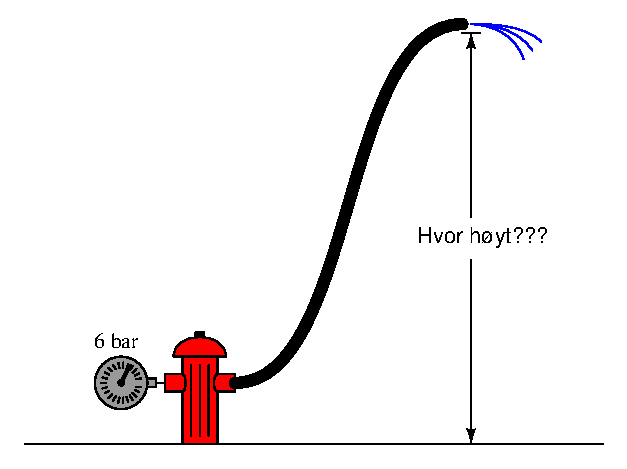
\includegraphics[width=15.5cm]{i00148x01.eps}$$

Anta nå at en stråledyse på slangeenden krever minst 2 bar trykk ved koblingen for å gi riktig vannstråle. Hvor høyt kan slangen løftes da, og fortsatt ha nok trykk ved dysen til brannslukking?

$$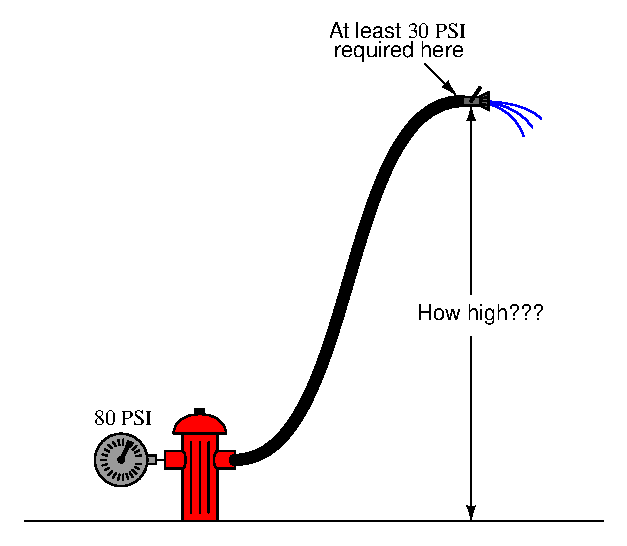
\includegraphics[width=15.5cm]{i00148x02.eps}$$

\vskip 20pt \vbox{\hrule \hbox{\strut \vrule{} {\bf Forslag til sokratisk diskusjon} \vrule} \hrule}

\begin{itemize}
\item{} Hvordan kan brannvesenet sikre at vannet kan sprøytes høyt nok ved brann i høye bygninger dersom hydranttrykket er utilstrekkelig?
\item{} Beskriv et scenario med denne brannslangen som illustrerer {\it Pascals prinsipp}.
\end{itemize}

\underbar{file i00148}
%(END_QUESTION)





%(BEGIN_ANSWER)

60.16 m og 40.77 m

\vskip 10pt

I praksis er dette en enhetskonvertering fra trykk til høyde vannsøyle. 80 PSI tilsvarer 184.54 fot vannsøyle, altså hvor høyt 80 PSI kan løfte en vannsøyle.

Med dyse på slangeenden kan vi bare «bruke opp» 50 PSI hydrostatisk trykk for å ha 30 PSI igjen ved dysen for korrekt funksjon. 50 PSI tilsvarer 115.33 fot, som dermed er maksimal høyde med dyse.

Det er viktig å forstå at første beregning ikke er særlig praktisk. 80 PSI ved hydranten vil {\it akkurat} løfte vann 184.54 fot. Hvis slangen var 190 fot og sto vertikalt, ville vannsøylen i slangen bli 184.54 fot høy, uten vann ut av toppen. Ved nøyaktig 184.54 fot ville vannet stå ved kanten, uten reell stråle. Derfor må praktisk høyde uten dyse være lavere enn 184.54 fot.

Scenarioet med dyse er mer realistisk, fordi vi får oppgitt et faktisk minimumstrykk ved slangeenden som må tas med i beregningen.

%(END_ANSWER)





%(BEGIN_NOTES)

%INDEX% Physics, static fluids: maximum height of fire hose

%(END_NOTES)
